\documentclass[10pt,a4paper]{article}

\usepackage[margin=0.9in]{geometry}
\usepackage[T1]{fontenc}
\usepackage{lmodern}
\usepackage{booktabs}
\usepackage{tabularx}
\usepackage{array}
\usepackage{enumitem}
\usepackage{amsmath}
\usepackage[hidelinks]{hyperref}
\usepackage{tikz}
\usetikzlibrary{arrows.meta,positioning,shapes.geometric,fit,calc}

\newcolumntype{Y}{>{\raggedright\arraybackslash}X}
\newcolumntype{L}[1]{>{\raggedright\arraybackslash}p{#1}}

% Breathing room between table rows, slightly tighter than the main paper
% because the tables here are long and the document is capped at five pages.
\setlength{\extrarowheight}{2.5pt}
\renewcommand{\arraystretch}{1.08}

\renewcommand{\thetable}{S\arabic{table}}
\renewcommand{\thefigure}{S\arabic{figure}}

\title{Supplementary Material for\\[4pt]
\large Biomedical Knowledge Graphs and Large Language Models:\\A Critical Engineering Survey}
\author{Rangan Das \and Sounak Ghosh \and Utsav Bandyopadhyay Maulik \and Sushmit Dasgupta
        \and Sanghamitra Bandyopadhyay \and Ujjwal Maulik}
\date{}

\begin{document}
\maketitle

\begin{abstract}
\noindent This document covers the reporting package for a graph-grounded language system, a scale
for grading reproducibility, a data card for a biomedical graph, the criteria for each step up the
evidence-maturity ladder, a privacy architecture, the signals worth monitoring after deployment,
and the limits of the standard benchmarks.
\end{abstract}

% =====================================================================
\section{What has to be pinned down}
\label{s:why}

Behavior here depends on a knowledge substrate that changes independently of the code. Construction
scripts for widely used biomedical graphs get revised after publication, terminologies issue
scheduled releases, and hosted model endpoints are replaced without notice. Two groups can run the
same published pipeline against the same named graph and get different answers, because one of them
downloaded it six months later.

So the artifact to specify is the configuration, not the model: $C = (M, P, G, T, R, V, I)$, being
the model and revision, the prompt and tool policy, the graph snapshot and schema, the terminology
releases, the retrieval policy, the verification layer, and the interface. Changing any element
produces a new system unless equivalence is shown.

Errors also do not stay local, which is what Fig.~\ref{fig:sfailure} shows. A wrong edge admitted at
construction is indexed like any other, retrieved when relevant, and cited accurately by a generator
with no way to know it is wrong.

\begin{figure}[!ht]
\centering
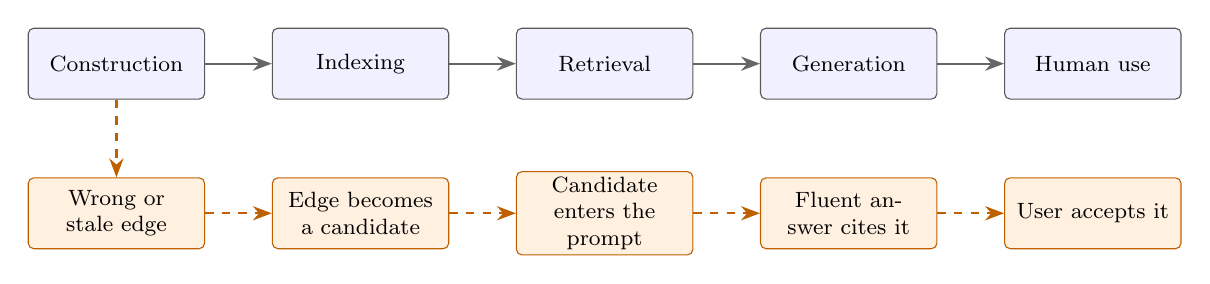
\begin{tikzpicture}[
  font=\footnotesize,
  st/.style={draw=black!65, rounded corners=2pt, fill=blue!6, text width=21mm,
             align=center, minimum height=9mm, inner sep=2pt},
  bad/.style={draw=orange!75!black, rounded corners=2pt, fill=orange!12, text width=21mm,
              align=center, minimum height=9mm, inner sep=2pt},
  a/.style={-{Stealth[length=2.4mm]}, thick, draw=black!60},
  b/.style={-{Stealth[length=2.4mm]}, thick, draw=orange!75!black, dashed}
]
\node[st] (c) at (0,0)      {Construction};
\node[st] (i) at (3.1,0)    {Indexing};
\node[st] (r) at (6.2,0)    {Retrieval};
\node[st] (g) at (9.3,0)    {Generation};
\node[st] (u) at (12.4,0)   {Human use};

\draw[a] (c) -- (i);
\draw[a] (i) -- (r);
\draw[a] (r) -- (g);
\draw[a] (g) -- (u);

\node[bad] (e1) at (0,-1.9)    {Wrong or stale edge};
\node[bad] (e2) at (3.1,-1.9)  {Edge becomes a candidate};
\node[bad] (e3) at (6.2,-1.9)  {Candidate enters the prompt};
\node[bad] (e4) at (9.3,-1.9)  {Fluent answer cites it};
\node[bad] (e5) at (12.4,-1.9) {User accepts it};

\draw[b] (e1) -- (e2);
\draw[b] (e2) -- (e3);
\draw[b] (e3) -- (e4);
\draw[b] (e4) -- (e5);
\draw[b] (c) -- (e1);
\end{tikzpicture}
\caption{\textbf{Why a single bad edge is hard to catch downstream.} The upper row is the intended
pipeline; the lower row follows one incorrect edge through it. Every step behaves correctly given its
input, so nothing raises an alarm. Reporting therefore has to cover provenance and snapshot identity,
not only model performance.}
\label{fig:sfailure}
\end{figure}

% =====================================================================
\section{The reporting package}
\label{s:artifacts}

What another group needs in order to reconstruct both the knowledge boundary and the retrieval
behavior of a published system. Table~\ref{tab:sreport} gives the items by category. Three deserve
emphasis. The graph is the part most often under-specified, and a schema that cannot express negation
or population drops them silently. Per-instance retrieval traces are the only way to tell a system that
retrieved the right evidence and misused it from one that never retrieved it. And if any evaluation
question was generated from the graph, that has to be stated, because agreement with the graph that
supplied the question is close to guaranteed.

\begin{table}[!ht]
\centering
\caption{\textbf{The reporting package, by category.} Each row lists what has to be released for that
part of the system to be reconstructable. The knowledge and retrieval rows are where published work most
often falls short, and they are also the rows that determine whether a reported result can be checked
for leakage after the fact.}
\label{tab:sreport}
\footnotesize
\begin{tabularx}{\textwidth}{@{}L{2.5cm} Y@{}}
\toprule
\textbf{Category} & \textbf{Report} \\
\midrule
Knowledge & Graph snapshot or a deterministic rebuild workflow, with checksums; schema including relation directionality and permitted qualifiers; every ontology and terminology release with edition and extension; source list with per-source versions and integration rules; licenses and redistribution constraints; graph statistics by node and relation type \\
Cohort and benchmark & Inclusion and exclusion criteria with the code that builds the cohort; index-time definition and split logic; exact benchmark release; lineage of any question generated from the graph, reported separately; contamination assessment against the model's training cutoff \\
Retrieval & Entity linker and version; embedding model and index version; query templates and every generated formal query; retrieval depth, reranking, context budget; retrieved node, edge, and path identifiers with scores per test instance; failure and timeout logs \\
Model & Exact identifier and revision, provider, access date; prompt templates and system messages; decoding parameters and context window; fine-tuning data and checkpoints where releasable \\
Evaluation & Raw outputs; atomic-claim decomposition and claim-to-evidence labels; automated judge model, version, prompts, and agreement with human labels on a calibration sample; clinician rubric, adjudication protocol, inter-rater agreement; analysis scripts, intervals, and all planned and exploratory outcomes \\
Operations & Environment with lockfile or container; run time, token use, cost assumptions; seeds and number of repeated runs \\
Change record & Graph updates, retractions, endpoint changes, prompt amendments, and benchmark corrections made after the experiment \\
\bottomrule
\end{tabularx}
\end{table}

Releasing a final answer and an aggregate metric makes retrieval error and circular evidence impossible
to audit, so the log needs a record per evaluation instance. Table~\ref{tab:srecord} gives the fields.
Where licensing or patient privacy prevents release, provide hashes, synthetic examples, access
instructions, and a data dictionary. Licensed terminology strings should not be redistributed beyond
their terms, and credentialed clinical data should never appear in a public trace.

\begin{table}[!ht]
\centering
\caption{\textbf{Fields for a per-instance evaluation record.} Each row is one field of a
machine-readable log entry written once per evaluation question. The purpose is to make every
reported score traceable to the evidence that produced it, so that a reviewer can distinguish a
retrieval failure from a reasoning failure without rerunning the system. The temporal and snapshot
fields are what allow a result to be checked for leakage after publication.}
\label{tab:srecord}
\footnotesize
\begin{tabularx}{\textwidth}{@{}L{4.6cm} Y@{}}
\toprule
\textbf{Field} & \textbf{Purpose} \\
\midrule
\texttt{question\_id}, \texttt{benchmark\_version} & Identifies the item and the exact release it came from \\
\texttt{patient\_or\_source\_group} & Supports clustered analysis and prevents split contamination \\
\texttt{index\_time} & Fixes the as-of boundary for any temporal claim \\
\texttt{graph\_snapshot} & Ties the answer to a specific knowledge state \\
\texttt{linked\_entities} & Exposes entity-linking error, the most common upstream failure \\
\texttt{executed\_queries} & Allows a reviewer to check semantic fidelity to the question \\
\texttt{retrieved\_nodes\_edges\_paths} & Separates retrieval failure from reasoning failure \\
\texttt{source\_documents\_and\_dates} & Enables citation entailment checking \\
\texttt{model\_and\_prompt\_version} & Identifies the generator configuration \\
\texttt{raw\_response} & Permits re-scoring under a different rubric \\
\texttt{atomic\_claims}, \texttt{claim\_evidence\_labels} & Support claim-level rather than answer-level accuracy \\
\texttt{final\_score} & The reported outcome for this item \\
\texttt{latency\_tokens\_cost} & Allows benefit to be normalized by resource use \\
\texttt{error\_category} & Makes failure analysis aggregable across instances \\
\bottomrule
\end{tabularx}
\end{table}

% =====================================================================
\section{Grading reproducibility}
\label{s:repro}

Reported as a binary, reproducibility loses information. A paper that describes an architecture and
releases nothing differs from one that releases code but omits the graph snapshot, and both differ from
one whose estimates an independent group has reproduced. Table~\ref{tab:srepro} grades these separately.

The top level is what matters for clinical claims. Reproducing a number on the same data shows the
pipeline was described accurately. Reproducing the direction and magnitude on a later time window,
another institution, or a newer snapshot shows the finding survives what actually changes in
deployment. Most current work reaches R1 or R2. Proprietary model use does not preclude a good grade,
but it requires dated identifiers, preserved raw outputs, repeated runs, and a plan for endpoint
retirement.

\begin{table}[!ht]
\centering
\caption{\textbf{A five-level scale for reporting how reproducible a study is.} The levels are
cumulative and describe evidence rather than intent, so a paper qualifies for a level only if
someone outside the author group could perform the corresponding action. R0 to R2 concern whether the
work can be rerun; R3 and R4 concern whether it survives being rerun. The gap between R2 and R3 is
where most published work currently stops, and the gap between R3 and R4 is what separates a
reproducible experiment from a durable finding.}
\label{tab:srepro}
\footnotesize
\begin{tabularx}{\textwidth}{@{}L{2.8cm} Y@{}}
\toprule
\textbf{Level} & \textbf{Criterion} \\
\midrule
R0 described & Architecture and results are described; data and code are unavailable. \\
R1 partially inspectable & Prompts or code are available, but the graph snapshot, retrieval traces, or model revision is missing. \\
R2 re-executable & Code, environment, accessible data, and a versioned graph together allow the published pipeline to be rerun. \\
R3 result reproducible & An independent rerun reproduces the main estimates within predeclared tolerances. \\
R4 transport reproduced & The direction and clinically material magnitude persist on a later time window, another institution, or a newer snapshot. \\
\bottomrule
\end{tabularx}
\end{table}

% =====================================================================
\section{A data card for a biomedical knowledge graph}
\label{s:datacard}

Naming a graph is not describing it. Two studies reporting the same well-known resource can differ in
snapshot date, terminology release, the proportion of edges that were curated rather than text-mined,
and the fraction of mentions that failed to resolve. Any of these changes the answer to a clinical
question, and none is visible from the resource name. Table~\ref{tab:sdatacard} asks for the
properties that determine what the graph can answer. Provenance, temporal coverage, and coverage over
the evaluated entities matter more than size, since four million relations are useless for a question
whose decisive entity is absent.

\begin{table}[!ht]
\centering
\caption{\textbf{Data card fields for a biomedical knowledge graph used in a language-model system.}
The fields are grouped by what they let a reader determine: whether they hold the same object as the
authors, what the graph's edges actually mean, whether an assertion can be traced and dated, whether
the graph covers the evaluated question, and what may lawfully be redistributed. A study that omits
the identity and provenance groups cannot be compared with another study on the same resource.}
\label{tab:sdatacard}
\footnotesize
\begin{tabularx}{\textwidth}{@{}L{2.6cm} Y@{}}
\toprule
\textbf{Group} & \textbf{Fields} \\
\midrule
Identity & Graph name, release, retrieval date, checksum, persistent identifier \\
Semantics & Node and relation schema, including directionality and permitted qualifiers \\
Composition & Upstream sources, source-specific versions, integration rules \\
Edge origin & Whether each relation is curated, rule-based, text-mined, inferred, or model-generated \\
Evidence & Claim-level provenance and how evidence strength is represented \\
Time & \texttt{valid\_from}, \texttt{valid\_to}, publication date, snapshot date \\
Coverage & Coverage over the evaluated entities, relations, and gold answers \\
Normalization & Ontology and terminology releases, mappings, unresolved-mention rate \\
Access & License, redistribution constraints, access procedure, permitted territories \\
Known bias & Demographic, geographic, linguistic, and publication skew \\
Maintenance & Update policy, retraction handling, supersession semantics \\
\bottomrule
\end{tabularx}
\end{table}

% =====================================================================
\section{What each step up the maturity ladder demands}
\label{s:gates}

Each gate tests a property the level below left unexamined, which is why a system can be excellent at
one level and fail at the next.

\paragraph{Gate A, analytical validity (E1 to E2).}
Freeze the whole configuration before testing. Compare against closed-book, long-context,
vector-retrieval, symbolic, and oracle-evidence arms, and evaluate the graph, retrieval, reasoning,
and generation stages separately. Use temporal splits. Report intervals and clinically weighted error
severity rather than accuracy alone, since a system that is slightly less accurate but never misses a
contraindication may be the better one.

\paragraph{Gate B, transportability (E2 to E3).}
Validate on an independent institution or a genuinely later period. Audit terminology mappings,
missing-data mechanisms, graph coverage, guideline version, subgroup performance, and calibration. A
fresh sample from the same pipeline is much weaker evidence than a changed population, because the
pipeline is often what the model learned.

\paragraph{Gate C, operational readiness (E3 to E4).}
In silent deployment, demonstrate availability, tail latency, timeout behavior, data freshness, safe
degradation, audit completeness, and incident detection. Complete privacy, security, safety, usability,
and regulatory assessment before any output reaches a user, since that is when a technical failure
becomes a clinical one.

\paragraph{Gate D, safe human use (E4 to E5).}
Predefine who may see, accept, reject, edit, or act on an output. Measure reliance, verification time,
alert burden, work redistribution, escalation, and the error types users fail to catch, which are not
the errors the system makes most often. Measure the work the system creates, not only the benefit.

\paragraph{Gate E, sustained benefit (E5 to E6).}
Establish comparative value, version-specific release criteria, monitoring thresholds, rollback
drills, incident review, and periodic independent audit. Revalidate after any material configuration
change. This gate never closes, which is why E6 is an operating state rather than an achievement.

% =====================================================================
\section{Designing for privacy when the graph is the disclosure risk}
\label{s:privacy}

A patient graph can be more disclosive than the record it came from. Linking a rare diagnosis to a
date, a location, a family relation, and a genomic variant can identify an individual after every
direct identifier is gone, because the combination narrows the population even when no single field
does. The attack surface extends past the graph to embeddings, vector indexes, cached prompts,
retrieved subgraphs, logs, and human feedback, all of which belong in the data inventory.

Legal obligations vary by jurisdiction, and meeting them is necessary rather than sufficient: a
compliance label does not stop a graph from leaking structure. Fig.~\ref{fig:sprivacy} gives the
architecture. Separate the population-level graph from patient graphs, authorize at query time against
the smallest subgraph that answers the question, and treat anything derived from a patient graph as
inheriting its sensitivity.

\begin{figure}[!ht]
\centering
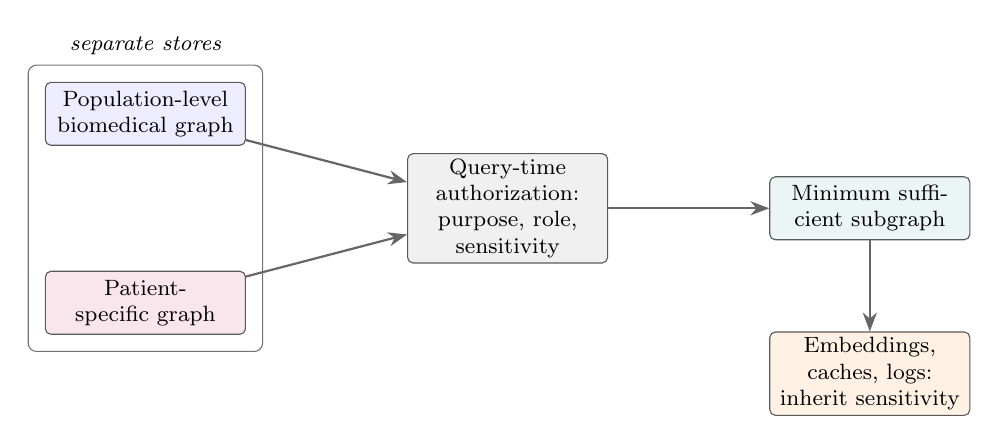
\begin{tikzpicture}[
  font=\footnotesize,
  zone/.style={draw=black!55, rounded corners=3pt, inner sep=6pt},
  n/.style={draw=black!65, rounded corners=2pt, text width=24mm, align=center,
            minimum height=8mm, inner sep=2pt},
  pub/.style={n, fill=blue!7},
  priv/.style={n, fill=purple!10},
  der/.style={n, fill=orange!10},
  a/.style={-{Stealth[length=2.4mm]}, thick, draw=black!60}
]
\node[pub] (global) at (0,0) {Population-level biomedical graph};
\node[priv] (patient) at (0,-2.4) {Patient-specific graph};
\node[n, fill=black!6] (authz) at (4.6,-1.2) {Query-time authorization: purpose, role, sensitivity};
\node[n, fill=teal!8] (sub) at (9.2,-1.2) {Minimum sufficient subgraph};

\node[der] (emb) at (9.2,-3.3) {Embeddings, caches, logs: inherit sensitivity};

\draw[a] (global) -- (authz);
\draw[a] (patient) -- (authz);
\draw[a] (authz) -- (sub);
\draw[a] (sub) -- (emb);

\node[zone, fit=(global)(patient), label={[font=\footnotesize\itshape]above:separate stores}] {};
\end{tikzpicture}
\caption{\textbf{Minimum privacy architecture for a patient-facing graph system.} The
population-level graph and patient graphs are kept in separate stores, so that a query cannot
traverse from one patient into another through a shared index. Authorization happens at query time
against purpose, role, and data sensitivity, rather than being applied as a filter after retrieval,
because a filter downstream of a retrieval that already crossed a boundary has nothing left to
protect. The orange node records the requirement that is most often overlooked: embeddings, caches,
and logs derived from a patient graph carry the same sensitivity as the graph, and therefore the same
retention limits and egress controls.}
\label{fig:sprivacy}
\end{figure}

The remaining controls are unglamorous. Encrypt in transit and at rest with key separation. Suppress
protected data from prompts, telemetry, and vendor retention unless explicitly authorized, and
document the data flow for every processor and model provider. Set retention limits for prompts,
retrieved context, embeddings, logs, and feedback. Filter output and control egress against
cross-patient disclosure. Provide auditable consent, access, correction, and deletion workflows where
they apply. Then attack the result with membership, reconstruction, and linkage tests. Federated
deployment reduces central data movement without guaranteeing privacy, since model updates,
gradients, graph statistics, and query patterns can each leak, so evaluate any privacy-enhancing
technology against a stated threat model rather than adopting it as a label.

% =====================================================================
\section{Monitoring a system whose knowledge keeps changing}
\label{s:monitoring}

A single accuracy measure is too slow and too coarse: too slow because it aggregates over a window,
too coarse because slack at one stage masks a deficit at another. A degradation that starts in the
graph will not show at the output for some time. Monitoring therefore has to be stage-local, and
Table~\ref{tab:smonitor} gives the signals.

What matters more than the list is what happens when a signal moves. Set every threshold in advance
and map it to a response: investigate, roll back, suspend, or fall back to a restricted mode. Rerun
sentinel cases after every material configuration change, since a series of individually harmless
updates can drift a system a long way without tripping any single threshold. For a dynamic evidence
graph, retrieve from approved immutable snapshots and promote a new one only after regression testing;
retrieving from a live graph means behavior changes without a release.

Incident response needs traceability both ways. From a harmful output back to the inputs, mappings,
retrieved edges, model, policy, and user actions. From a corrupted source forward to every release and
output that depended on it. A system with only the first can explain one failure and cannot bound its
blast radius.

\begin{table}[!ht]
\centering
\caption{\textbf{Post-deployment monitoring signals, grouped by pipeline stage.} The grouping mirrors
the evaluation layers of the main paper so that a monitoring alert points at a stage rather than at
the system as a whole. Signals in the upper rows are leading indicators: unmapped concepts and
retraction backlog move before answer quality does, which is what makes them worth instrumenting.
Signals in the lower rows are lagging but decisive, since a rise in override rate or adverse events
is evidence that earlier thresholds were set too loosely.}
\label{tab:smonitor}
\footnotesize
\begin{tabularx}{\textwidth}{@{}L{3.0cm} Y@{}}
\toprule
\textbf{Stage} & \textbf{Signals} \\
\midrule
Input and mapping & Missingness, out-of-range values, unmapped concepts, ambiguity rate, language and site shift \\
Graph & Source freshness, retractions processed, provenance completeness, schema violations, edge-confidence distribution, update failures \\
Retrieval & No-evidence rate, sentinel-case recall, graph-versus-text source mix, contraindication retrieval, subgraph size, latency \\
Generation and verification & Unsupported-claim rate, citation entailment, contradiction rate, abstention rate, verifier disagreement, unsafe fallback events \\
Human use & Acceptance, override, and edit rates, verification time, automation-bias indicators, workarounds, complaints, near misses \\
Outcome and equity & Task success, adverse events, workflow time, decision changes, subgroup calibration and error severity \\
Operations and security & Availability, tail latency, timeouts, cost, access anomalies, injection attempts, data-leakage indicators, unauthorized changes \\
\bottomrule
\end{tabularx}
\end{table}

% =====================================================================
\section{Where the standard benchmarks mislead}
\label{s:benchmarks}

Each benchmark measures something narrower than its name suggests, so no single one validates a
graph-grounded clinical system. Extraction benchmarks do not establish the accuracy of the integrated
graph. Link prediction does not establish that a novel hypothesis is true, still less that a drug
works. Medical question answering does not establish workflow performance, patient outcomes, or freedom
from memorization. Retrieval benchmarks do not isolate a graph-derived benefit without a matched
text-retrieval arm. Graph-comprehension benchmarks say nothing about clinical validity. Domain graph
reasoning agrees with a source graph, errors included. Temporal and contamination-resistant benchmarks
are early evidence, not prospective safety.

Three mismatches recur. \emph{Task mismatch} is using exam-style question answering to support a claim
about clinical diagnosis, or link prediction to support one about drug efficacy; the benchmark is fine,
the inference is not. \emph{Knowledge mismatch} is generating evaluation questions from the same graph
supplied at inference, which makes agreement nearly automatic and says little about correctness beyond
it. \emph{Interface mismatch} is serializing graph facts in a format that suits one model family, then
reporting the result as a property of the method rather than of the pairing.



% =====================================================================
\section{Leakage}
\label{s:leakage}

Most leakage routes here inflate the graph arm rather than both arms equally, which makes leakage a
threat to the attribution of the benefit and not just its size. If evaluation questions were generated
from the inference graph, the graph arm is scored on reconstructing its own input while the closed-book
arm is not. The measured benefit is then an artifact of the design, and no downstream statistical care
recovers from it.

Table~\ref{tab:sleak} lists the mechanisms and controls. Two have no analogue in conventional
evaluation. \emph{Ontology leakage} occurs when a label sits in the definitions or synonyms supplied to
the model, turning classification into lookup. \emph{Model-mediated circularity} occurs when one model
family builds the edges, writes the questions, answers them, and judges the answers; correlated errors
then read as agreement, and self-consistency checks amplify rather than detect it.

The concern is empirical. Models trained with medically harmful misinformation retained ordinary
benchmark performance, so the benchmarks missed a clinically important degradation, and removing
train-test redundancies changes embedding-model results on biomedical graphs. A random held-out edge
does not simulate future discovery.

\begin{table}[!ht]
\centering
\caption{\textbf{Leakage mechanisms, their consequences, and the controls that address them.} Each row
is a distinct route by which information about the answer reaches the system before it should. The
mechanisms are ordered roughly from most to least widely recognized, and the last four are specific to
graph-grounded systems. Most of these routes inflate the graph arm without inflating the baseline, which
is why leakage here threatens the attribution of the benefit and not merely the size of it.}
\label{tab:sleak}
\footnotesize
\begin{tabularx}{\textwidth}{@{}L{3.0cm} Y Y@{}}
\toprule
\textbf{Mechanism} & \textbf{Consequence} & \textbf{Control} \\
\midrule
Parametric benchmark contamination & Inflated closed-book scores; the retrieval effect becomes uninterpretable & Post-cutoff or private evaluation; report cutoff and API date; memorization probes; include a no-context arm \\
Hyperparameter and test reuse & Reported gains reflect adaptation to the test set & Freeze a development set; preregister the comparison; evaluate once on held-out data \\
Patient or encounter leakage & Models exploit patient identity or post-outcome information & Split by patient; define index time; censor features and edges; audit timestamps \\
Temporal leakage & Retrospective performance overstates real-time capability & Freeze all sources at the prediction date; use temporal splits; distinguish valid from transaction time \\
Graph-to-answer leakage & The system reconstructs its input resource rather than independent truth & Independently authored questions; disclose generation lineage; report graph-derived and external items separately \\
Inverse or redundant relations & Link-prediction scores measure trivial reconstruction & Remove inverse, symmetric, duplicate, and logically entailed test edges \\
Ontology leakage & Classification degenerates into label lookup & Redact label-bearing fields; measure lexical overlap; evaluate unseen concepts \\
Model-mediated circularity & Correlated model errors appear as agreement & Separate construction, generation, and judging models; use human adjudication; retain disagreement \\
\bottomrule
\end{tabularx}
\end{table}

\end{document}
